\documentclass[conference]{IEEEtran}
\IEEEoverridecommandlockouts
\usepackage{cite}
\usepackage{amsmath,amssymb,amsfonts}
\usepackage{graphicx}
\usepackage{textcomp}
\usepackage{xcolor}
\usepackage{subcaption}
\usepackage{url}
\usepackage{hyperref}
\usepackage{booktabs} % Para mejores tablas
% TeX Live ``basic'' a veces no incluye Courier (pcr); usar cmtt para \texttt
\renewcommand{\ttdefault}{cmtt}
\def\BibTeX{{\rm B\kern-.05em{\sc i\kern-.025em b}\kern-.08em
    T\kern-.1667em\lower.7ex\hbox{E}\kern-.125emX}}
\begin{document}

\title{Proyecto I: Reconocimiento de comandos de voz y
despliegue móvil con ONNX Runtime Mobile}

\author{\IEEEauthorblockN{Fabricio Mena Mejía}
\IEEEauthorblockA{Instituto Tecnológico de Costa Rica\\
Email: fabriciomena11@estudiantec.cr}
\and
\IEEEauthorblockN{Anthony Fuentes Calvo}
\IEEEauthorblockA{Instituto Tecnológico de Costa Rica\\
Email: anthonyfuentescalvo@estudiantec.cr}
\and
\IEEEauthorblockN{Fernando Sánchez Hidalgo}
\IEEEauthorblockA{Instituto Tecnológico de Costa Rica\\
Email: Fer.sanchez@estudiantec.cr}}

\maketitle

\begin{abstract}
Este informe corresponde al Proyecto~I del curso de Inteligencia Artificial: se construye, de extremo a extremo, un reconocedor de comandos de voz de vocabulario reducido orientado a un escenario de asistencia o control (p.\,ej.\ hogar inteligente), pasando del dato crudo al despliegue en dispositivo. Siguiendo el enunciado, se adopta el conjunto público \textit{Google Speech Commands} v0.02 con diez clases, partición oficial de entrenamiento, validación y prueba, y una representación tipo imagen mediante mel-espectrograma normalizado y reescalado a $128 \times 128$ para alimentar redes convolucionales en PyTorch. Se comparan dos familias de modelos---LeNet-5 adaptado (con \texttt{Tanh}) y MobileNetV2 en una variante ligera---bajo datos crudos frente a datos aumentados (desplazamiento temporal, ruido y SpecAugment) y tres configuraciones de hiperparámetros por combinación, lo que produce doce entrenamientos comparables. Las métricas en prueba muestran superioridad sostenida de MobileNetV2 (hasta $0.9633$ de exactitud en la mejor corrida). El seguimiento experimental se centralizó en Weights \& Biases. Por último, se documenta la línea de trabajo hacia la exportación ONNX, la comprobación de paridad con respecto a PyTorch y la integración prevista con ONNX Runtime Mobile en una aplicación Android (Jetpack Compose) que mapea la predicción a acciones de interfaz.
\end{abstract}

\begin{IEEEkeywords}
Comandos de voz, mel-espectrograma, redes neuronales convolucionales, aumentación de datos, Weights \& Biases, ONNX, ONNX Runtime Mobile.
\end{IEEEkeywords}

\section{Marco teórico}

La clasificación de audio corto puede formularse como reconocimiento de patrones en una imagen tiempo-frecuencia: a partir de una forma de onda muestreada se calcula una transformada de Fourier de tiempo corto (STFT) y un banco de filtros mel que aproxima la percepción humana de tono; el logaritmo de la energía mel amortigua la dinámica y facilita el entrenamiento de redes profundas \cite{torchaudio_docs}. Las redes neuronales convolucionales (CNN) en dos dimensiones extraen jerarquías locales de texturas y formas en ese mapa, de forma análoga a la visión por computador aplicada a representaciones espectrales.

Para mejorar la generalización bajo ruido y variaciones de canal, es habitual aplicar aumentación en el dominio del tiempo (p.\,ej.\ desplazamiento) y en el espectro; SpecAugment enmascara franjas de tiempo y frecuencia en el mel-espectrograma durante el entrenamiento, obligando al modelo a no depender de un único bin o frame \cite{specaugment}.

En dispositivos móviles, conviene separar entrenamiento (PyTorch) e inferencia ligera: exportar el grafo a ONNX en modo evaluación, con pesos congelados, y ejecutarlo con ONNX Runtime Mobile reduce dependencias y habilita optimizaciones de tiempo de ejecución \cite{onnxruntime}. La calidad del despliegue exige que el preprocesamiento en el terminal replique fielmente el usado al entrenar; la discrepancia se controla con pruebas de paridad logit-a-logit entre PyTorch y el runtime ONNX \cite{onnxruntime}.

\section{Dataset y preprocesamiento}

\subsection{Speech Commands v0.02 y subconjunto de diez clases}
Se utilizó el conjunto \textit{Speech Commands} v0.02 distribuido por TensorFlow Datasets \cite{tensorflow_datasets_speech_commands}, compuesto por grabaciones en formato WAV de un segundo o menos, organizadas en carpetas por etiqueta léxica. Siguiendo el alcance del proyecto, se trabajó con diez comandos: \texttt{yes}, \texttt{no}, \texttt{up}, \texttt{down}, \texttt{left}, \texttt{right}, \texttt{on}, \texttt{off}, \texttt{stop} y \texttt{go}.

\subsection{División entrenamiento, validación y prueba}
La partición oficial del corpus se respeta mediante los archivos \texttt{validation\_list.txt} y \texttt{testing\_list.txt} incluidos en la raíz del dataset: las rutas listadas en ellos definen los conjuntos de validación y de prueba, respectivamente. El entrenamiento comprende el resto de archivos \texttt{.wav} de las diez clases que no aparecen en dichas listas, lo que garantiza que no haya solapamiento de hablantes ni clips entre particiones y que los resultados sean comparables con la literatura.

\subsection{Representación tipo imagen y flujo reproducible}
Cada clip se re-muestrea a mono PCM de 16\,kHz y se recorta o rellena a una ventana fija de un segundo antes del análisis espectral. En el cuaderno de entrenamiento (\texttt{proy1.ipynb}) la STFT utiliza \texttt{n\_fft}=1024, \texttt{hop\_length}=256 y \texttt{n\_mels}=128; el mel-espectrograma en escala logarítmica se normaliza por muestra y se re-escala espacialmente a $128 \times 128$, produciendo tensores de forma $(1,128,128)$ compatibles con las entradas descritas en las Tablas~\ref{tab:arquitectura} y~\ref{tab:arquitectura_b}. Herramientas auxiliares del repositorio documentan además un contrato de preprocesamiento alternativo (p.\,ej.\ otros tamaños de FFT) orientado a paridad con tiempo de ejecución ligero; cualquier despliegue debe fijar un único contrato y ceñirse a él de extremo a extremo.

La reproducibilidad se apoya en la semilla global 42 (v\'ease el control de aleatoriedad en la siguiente secci\'on), en el uso determinista de las listas oficiales de validaci\'on y prueba y en la trazabilidad de hiperpar\'ametros y curvas en Weights \& Biases.

\section{Diseño de arquitectura de IA}

\subsection{Control de Aleatoriedad y Reproducibilidad}
Para garantizar la reproducibilidad de los experimentos, se implementó un estricto control de aleatoriedad. Se definió una semilla global (\textit{seed} $= 42$) utilizada para inicializar los generadores de números pseudoaleatorios de las librerías \texttt{random}, \texttt{numpy} y \texttt{torch}. Adicionalmente, se configuró el comportamiento determinista de cuDNN desactivando el \textit{benchmark} dinámico donde fuera necesario.

\subsection{Selección de Técnicas de Aumentación de Datos}
Para mejorar la capacidad de generalización de los modelos y simular condiciones realistas de entorno (ruido de fondo, variabilidad de hablantes), se aplicaron técnicas de aumento de datos (\textit{data augmentation}) en el preprocesamiento de audio. Las técnicas se inspiraron en métodos avanzados de aumento espectral y en el dominio del tiempo:
\begin{itemize}
    \item \textbf{Time Shift:} Desplazamiento temporal aleatorio para que el sistema aprenda predicciones invariantes al milisegundo exacto de reproducción, alineándose directamente con aplicaciones reales bajo ruidos dispares.
    \item \textbf{Ruido Blanco (White Noise):} Inyectado progresivamente para simular grabaciones en ambientes no controlados y servir de fuerte regularización matemática de los tensores.
    \item \textbf{SpecAugment \cite{specaugment}:} Enmascaramiento de bloques de frecuencias y tiempo directamente sobre el mel-espectrograma para forzar a la red neuronal a no depender de características auditivas frágiles y lograr márgenes más robustos.
\end{itemize}

\subsection{Modelo A: LeNet-5 Adaptado}
El Modelo A está basado en la arquitectura clásica de LeNet-5, pero fue adaptado específicamente para el procesamiento de mel-espectrogramas.

\subsubsection{Justificación de modificaciones}
Se realizaron los siguientes cambios sobre la arquitectura original de LeCun:
\begin{itemize}
    \item \textbf{Tamaño de entrada:} Se modificó para recibir tensores de $1 \times 128 \times 128$ correspondientes a las imágenes generadas del audio, en lugar de los $32 \times 32$ originales.
    \item \textbf{Filtros convolucionales:} Se aumentó el número de canales a 32, 64 y 128 en las tres capas convolucionales consecutivas para capturar patrones espectrales más ricos y complejos.
    \item \textbf{Función de Activación:} Se preserva el uso de la función de activación clásica \texttt{Tanh} estipulada en la arquitectura original de LeNet-5. Esto se hace en estricto cumplimiento con los requerimientos del proyecto que limitan el uso de funciones más modernas como \texttt{ReLU}, garantizando así que el modelo mantenga la esencia matemática clásica de la red mientras se adapta al dominio de audio.
    \item \textbf{Padding:} En las capas convolucionales iniciales se utiliza un \texttt{padding=0}, consistentemente con la versión clásica de LeNet. Esta elección genera una reducción espacial después de cada convolución antes del \texttt{AvgPool2d}, lo que simplifica el diseño y mantiene la estructura de extracción de características sin introducir ceros adicionales en los bordes.
    \item \textbf{Clasificador 100\% Convolucional:} Se reemplazó la sección tradicional de capas totalmente conectadas (\textit{Fully Connected}) por una operación de \textit{Global Average Pooling} seguida de convoluciones $1 \times 1$. Esta modificación reduce significativamente el número de parámetros y mitiga el sobreajuste (\textit{overfitting}), preparando el modelo para su futuro despliegue en dispositivos móviles donde los parámetros en capas densas consumen demasiada memoria RAM.
\end{itemize}

\subsubsection{Definición de la Arquitectura}
La arquitectura final se resume en el diagrama presentado en la Tabla \ref{tab:arquitectura}. Consta de tres bloques convolucionales iniciales con \textit{Average Pooling}, seguidos de una capa de \textit{Global Average Pooling} y un bloque clasificador compuesto exclusivamente por convoluciones de $1 \times 1$.

\begin{table}[htbp]
\caption{Diagrama de Capas - LeNet-5 Adaptado}
\label{tab:arquitectura}
\centering
\begin{tabular}{ll}
\toprule
\textbf{Capa / Operación} & \textbf{Dimensión de Salida} \\
\midrule
Input (Mel-Spectrogram) & $(B, 1, 128, 128)$ \\
Conv1 ($32 \times 5 \times 5$) + Tanh + AvgPool(2) & $(B, 32, 62, 62)$ \\
Conv2 ($64 \times 5 \times 5$) + Tanh + AvgPool(2) & $(B, 64, 29, 29)$ \\
Conv3 ($128 \times 5 \times 5$) + Tanh + AvgPool(2) & $(B, 128, 12, 12)$ \\
Global Average Pooling & $(B, 128, 1, 1)$ \\
Conv4 ($128 \to 512, 1 \times 1$) + Tanh & $(B, 512, 1, 1)$ \\
Conv5 ($512 \to 128, 1 \times 1$) + Tanh & $(B, 128, 1, 1)$ \\
Conv6 ($128 \to 10, 1 \times 1$) (Logits) & $(B, 10, 1, 1)$ \\
Flatten Final & $(B, 10)$ \\
\bottomrule
\end{tabular}
\end{table}

\begin{figure}[htbp]
\centerline{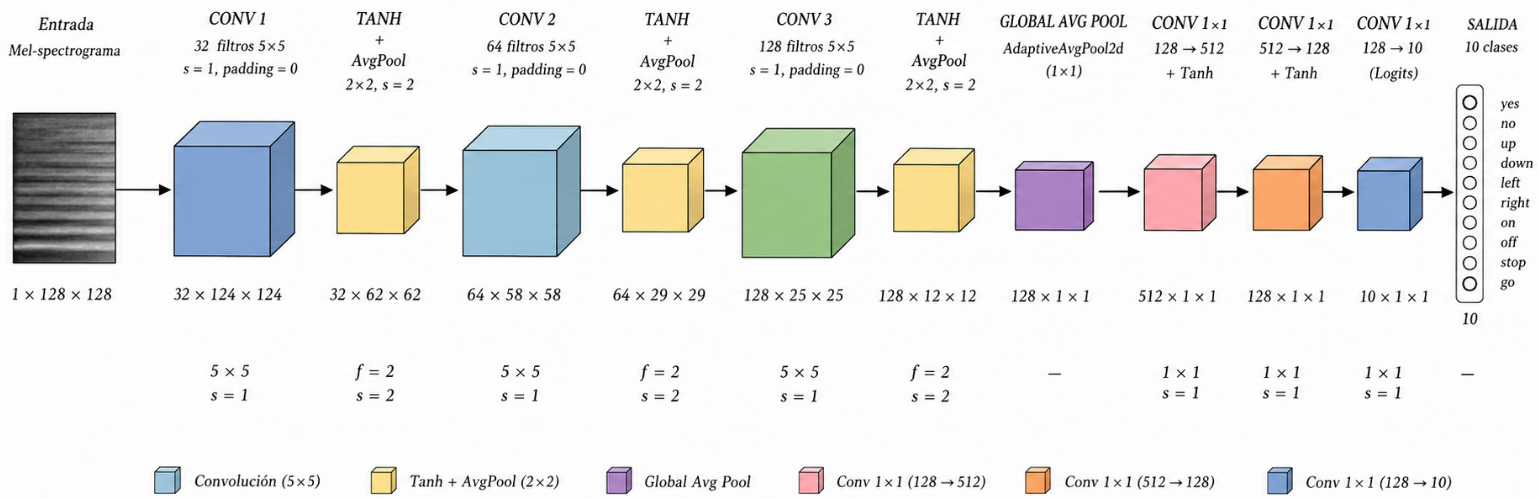
\includegraphics[width=\linewidth]{images/Modelo_LeNet5_adaptado.png}}
\caption{Diagrama visual de la arquitectura del Modelo A.}
\label{fig:model_a}
\end{figure}

\subsubsection{Función de Pérdida, Optimizador y Entrenamiento}
Se utilizó \textit{Cross-Entropy Loss} como función de pérdida, la cual es ideal para clasificación multiclase. El optimizador seleccionado fue \texttt{Adam} con una tasa de aprendizaje de $1 \times 10^{-3}$ y \textit{weight decay} de $1 \times 10^{-4}$ para mitigar el sobreajuste. Además, se empleó un \textit{scheduler} (\texttt{ReduceLROnPlateau}) que reduce la tasa de aprendizaje a la mitad si la precisión de validación no mejora en 3 épocas. Las rutinas de entrenamiento se ejecutaron usando precisión mixta nativa (\texttt{torch.amp}).


\subsection{Modelo B: MobileNetV2 Adaptado}
El Modelo B está basado en la arquitectura de MobileNetV2, reconocida por su alta eficiencia y bajo consumo de parámetros en dispositivos móviles. Esta red fue programada de manera estructurada y adaptada específicamente para la clasificación de audio mediante espectrogramas de Mel.

\subsubsection{Justificación de modificaciones}
Se instrumentaron los siguientes cambios respecto a la arquitectura estándar de MobileNetV2 para adaptarla plenamente al dominio de audio:
\begin{itemize}
    \item \textbf{Tamaño de entrada y 1 Canal:} La capa convolucional inicial (que utiliza un bloque de \textit{Conv2d + BatchNorm + ReLU6}) recibe un tensor adaptado a un solo canal, correspondiente a imágenes en escala de grises de mel-espectrogramas ($1 \times 128 \times 128$), en contraste con los comunes $3 \times 224 \times 224$ (RGB) de ImageNet.
    \item \textbf{Uso de Inverted Residuals:} Se conservó la topología matricial de bloques convolucionales de tipo \textit{Inverted Residual} provista por redes móviles con convoluciones mutuamente separables (\textit{Depthwise Separable Convolutions}), con el propósito fundamental de reducir a niveles infimos el costo de operaciones en hardware móvil.
    \item \textbf{Clasificador Lineal y Reducción de Ruido:} El tensor de la extracción de características finaliza su procesamiento en una capa \textit{Global Average Pooling}. A continuación se aplica una capa reguladora \textit{Dropout} ($p=0.2$) para estabilizar la varianza, resolviendo hacia una sola capa lineal enfocada a clasificar los comandos correspondientes.
\end{itemize}

\subsubsection{Definición de la Arquitectura}
La secuencia en su estructura se presenta en la Tabla \ref{tab:arquitectura_b}. Consiste en un bloque inicial expansivo, siete etapas secuenciadas que usan estructuras \textit{Inverted Residual} con distintas profundidades en factor ($t$, $c$, $n$, $s$) para extracción iterativa y eficiente, así como un último subconjunto con promediado de vectores lineales.

\begin{table}[htbp]
\caption{Diagrama de Capas - MobileNetV2 Adaptado}
\label{tab:arquitectura_b}
\centering
\begin{tabular}{ll}
\toprule
\textbf{Capa / Operación} & \textbf{Dimensión / Canal} \\
\midrule
Input (Mel-Spectrogram) & $(B, 1, 128, 128)$ \\
Conv1 ($1 \to 32, 3 \times 3$) + BN + ReLU6 & $(B, 32)$ \textit{Stride 2}\\
Inverted Residual 1 ($t=1, c=16, n=1, s=1$) & $(B, 16)$ \\
Inverted Residual 2 ($t=6, c=24, n=2, s=2$) & $(B, 24)$ \\
Inverted Residual 3 ($t=6, c=32, n=3, s=2$) & $(B, 32)$ \\
Inverted Residual 4 ($t=6, c=64, n=4, s=2$) & $(B, 64)$ \\
Inverted Residual 5 ($t=6, c=96, n=3, s=1$) & $(B, 96)$ \\
Inverted Residual 6 ($t=6, c=160, n=3, s=2$) & $(B, 160)$ \\
Inverted Residual 7 ($t=6, c=320, n=1, s=1$) & $(B, 320)$ \\
Conv Pointwise (1x1) + BN + ReLU6 & $(B, 1280)$ \\
Global Average Pooling & $(B, 1280)$ \\
Dropout ($p=0.2$) + Linear ($1280 \to 10$) & $(B, 10)$ \\
\bottomrule
\end{tabular}
\end{table}

\begin{figure}[htbp]
\centerline{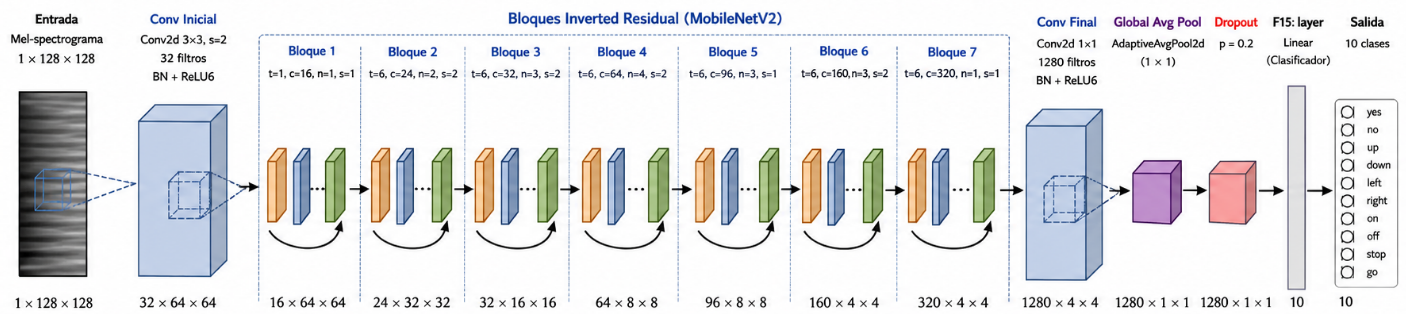
\includegraphics[width=\linewidth]{images/Modelo_MobileNetV2_adaptado.png}}
\caption{Diagrama visual de la arquitectura del Modelo B.}
\label{fig:model_b}
\end{figure}

\subsubsection{Función de Pérdida, Optimizador y Entrenamiento}
Del mismo modo que en el modelo A, se adoptó como función de pérdida la \textit{Cross-Entropy Loss} al ser la más robusta para clases multivariadas. Respecto a la optimización, se ajustó al uso del algoritmo \texttt{Adam}, manteniendo ratios controlados bajo reducción (\textit{Weight Decay} y un programa de control \texttt{ReduceLROnPlateau}) aprovechando implementaciones de cálculo por precisión geométrica (\texttt{torch.amp}) para reducir la memoria total GPU.

\section{Análisis y comparación de resultados}

\subsection{Registro de experimentos con Weights \& Biases}
Para cumplir con la rúbrica de trazabilidad, cada una de las doce corridas de entrenamiento se instrumentó con Weights \& Biases (W\&B) \cite{wandb}: por época se registraron, entre otras, la pérdida de entrenamiento, la exactitud y el F1 macro en validación, y al finalizar el entrenamiento las métricas agregadas en el conjunto de prueba junto con la matriz de confusión como imagen. Los proyectos y tableros permiten comparar curvas entre configuraciones y entre variantes con y sin aumentación.

En el cuaderno de entrenamiento, las corridas de ambos modelos se registraron bajo el mismo proyecto W\&B \url{https://wandb.ai/fabriciomenamejia-tec-costa-rica/speech-commands-model-a}, diferenciadas por el nombre de cada \textit{run} (p.\,ej.\ \texttt{modelo-a-raw-config1}, \texttt{modelo-b-augmented-config2}).

\begin{figure}[htbp]
\centerline{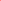
\includegraphics[width=\linewidth]{images/wandb_dashboard_overview.png}}
\caption{Vista del proyecto en Weights \& Biases: métricas por corrida.}
\label{fig:wandb}
\end{figure}

La Tabla~\ref{tab:doce_runs} consolida en una sola vista los resultados de \textit{test} de los doce entrenamientos (dos arquitecturas $\times$ dos regímenes de datos $\times$ tres configuraciones de hiperparámetros), alineados con las tablas detalladas en las subsecciones posteriores.

\begin{table*}[t]
\caption{Métricas en el conjunto de prueba: las doce corridas experimentales.}
\label{tab:doce_runs}
\centering
{\footnotesize
\begin{tabular}{@{}lllccc@{}}
\toprule
\textbf{Modelo} & \textbf{Datos} & \textbf{Cfg} & \textbf{Accuracy} & \textbf{F1 macro} & \textbf{Loss} \\
\midrule
A (LeNet-5) & crudos & 1 & 0.6388 & 0.6344 & 1.0522 \\
A (LeNet-5) & crudos & 2 & 0.8883 & 0.8880 & 0.3475 \\
A (LeNet-5) & crudos & 3 & 0.7074 & 0.7034 & 0.8022 \\
A (LeNet-5) & aumentados & 1 & 0.8271 & 0.8262 & 0.5050 \\
A (LeNet-5) & aumentados & 2 & 0.8322 & 0.8316 & 0.4863 \\
A (LeNet-5) & aumentados & 3 & 0.8016 & 0.8004 & 0.5796 \\
B (MobileNetV2) & crudos & 1 & 0.9592 & 0.9590 & 0.1826 \\
B (MobileNetV2) & crudos & 2 & 0.9552 & 0.9551 & 0.2073 \\
B (MobileNetV2) & crudos & 3 & 0.9633 & 0.9631 & 0.1430 \\
B (MobileNetV2) & aumentados & 1 & 0.9497 & 0.9493 & 0.2317 \\
B (MobileNetV2) & aumentados & 2 & 0.9435 & 0.9430 & 0.2534 \\
B (MobileNetV2) & aumentados & 3 & 0.9507 & 0.9503 & 0.1523 \\
\bottomrule
\end{tabular}
}
\end{table*}

\subsection{Modelo A: Datos crudos}

Para evaluar rigurosamente la arquitectura LeNet-5 adaptada a mel-espectrogramas con el uso de datos crudos (sin aumento), se diseñaron iteraciones con tres configuraciones de hiperparámetros distintas durante la fase de entrenamiento:

\begin{itemize}
    \item \textbf{Configuración 1:} Tasa de aprendizaje (LR) de $1 \times 10^{-3}$, tamaño de lote (BS) de 128, y manejador \texttt{ReduceLROnPlateau} (factor=0.5, patience=3).
    \item \textbf{Configuración 2:} Tasa de aprendizaje de $5 \times 10^{-4}$, tamaño de lote de 64, y el programador \texttt{StepLR} (step\_size=10, gamma=0.5).
    \item \textbf{Configuración 3:} Tasa de aprendizaje más alta de $2 \times 10^{-3}$, tamaño de lote de 256, y \texttt{ReduceLROnPlateau} más agresivo (factor=0.3, patience=5).
\end{itemize}

Los resultados globales consolidados para cada ensayo sobre el conjunto de prueba (Test) se registran en la Tabla \ref{tab:metricas_a_configs}.

\begin{table}[htbp]
\caption{Resultados por Configuración - Modelo A (datos crudos)}
\label{tab:metricas_a_configs}
\centering
\begin{tabular}{lccc}
\toprule
\textbf{Configuración} & \textbf{Accuracy} & \textbf{F1-Score (Macro)} & \textbf{Loss} \\
\midrule
Configuración 1 & 0.6388 & 0.6344 & 1.0522 \\
Configuración 2 & \textbf{0.8883} & \textbf{0.8880} & \textbf{0.3475} \\
Configuración 3 & 0.7074 & 0.7034 & 0.8022 \\
\bottomrule
\end{tabular}
\end{table}

A partir de las métricas expuestas, es evidente que la \textbf{Configuración 2} resulta ser el mejor modelo. Al combinar una tasa de aprendizaje moderada con un menor tamaño de lote (64) y reducciones escalonadas (\texttt{StepLR}), el modelo evitó caer tempranamente en mínimos locales u oscilar sin convergencia, mejorando considerablemente su generalización sobre los audios y logrando acercarse a una precisión de prueba rondando un 89\%. 

Al aislar el análisis sobre este mejor modelo (Configuración 2), se evaluaron sus gráficas de rendimiento.

\begin{figure}[htbp]
\centerline{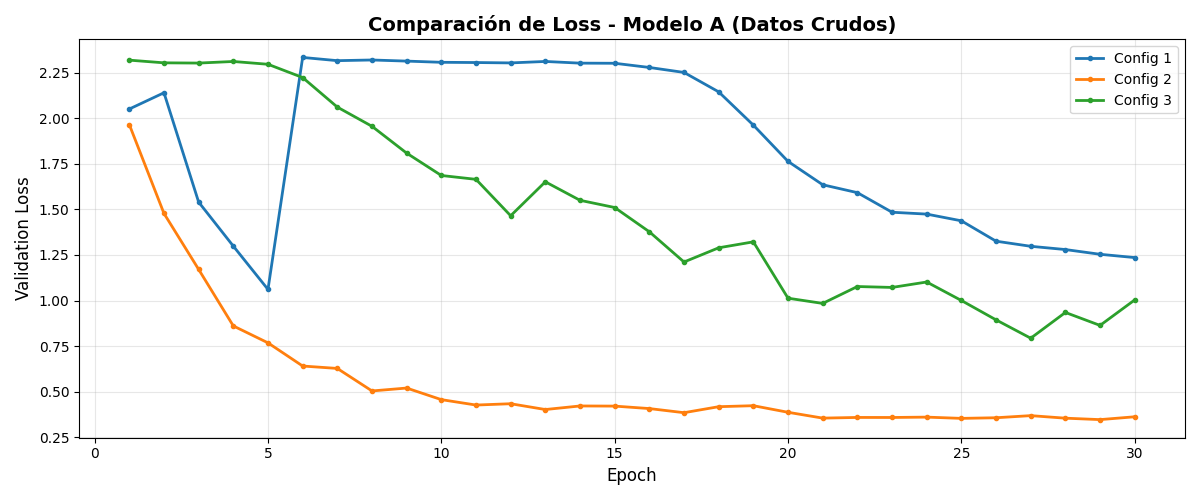
\includegraphics[width=\linewidth]{images/Grafica_Loss_Modelo_A_raw.png}}
\caption{Pérdida de entrenamiento y validación para el mejor Modelo A (Configuración 2).}
\label{fig:loss_a}
\end{figure}

En la gráfica de \textbf{Loss}, la curva de entrenamiento y la de validación descienden de manera más rápida y progresiva en comparación a configuraciones truncadas, acercándose asintóticamente a un valor inferior a 0.4. El uso de \texttt{StepLR} garantiza descensos estables a través del tiempo de cómputo, indicando menos señales de sobreajuste drástico durante casi todas las épocas.

\begin{figure}[htbp]
\centerline{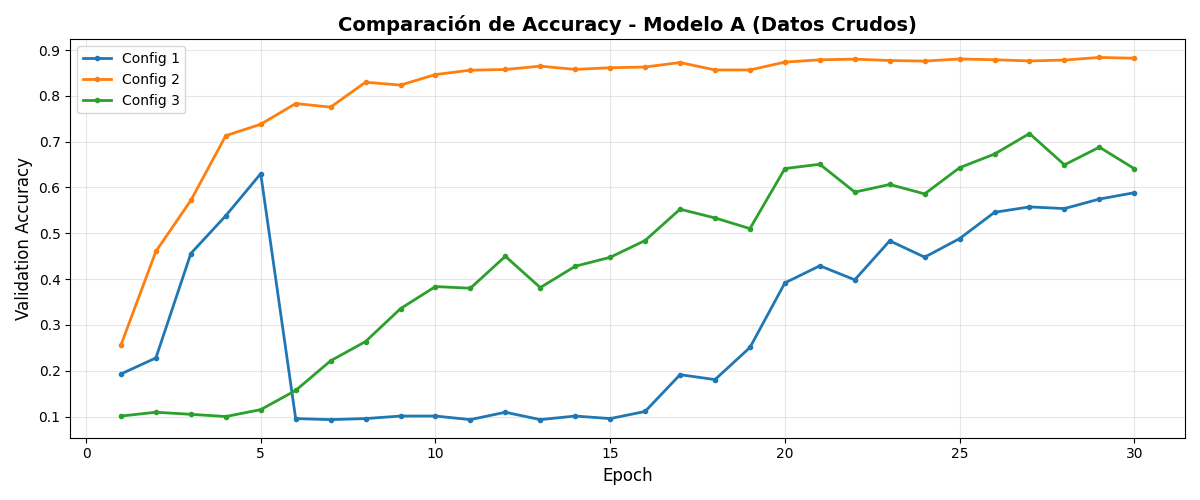
\includegraphics[width=\linewidth]{images/Grafica_Accuracy_Modelo_A_raw.png}}
\caption{Precisión de entrenamiento y validación para el mejor Modelo A (Configuración 2).}
\label{fig:accuracy_a}
\end{figure}

Al examinar la gráfica de \textbf{Accuracy}, el modelo exhibe un aprendizaje firme. Muestra crecimientos significativos durante las primeras 15 épocas estabilizándose gradualmente hacia el \textasciitilde 88-89\%. La reducción de escalón en la época 10 consolida esta precisión impidiendo inestabilidades en la fase final de ajuste.

\begin{figure}[htbp]
\centerline{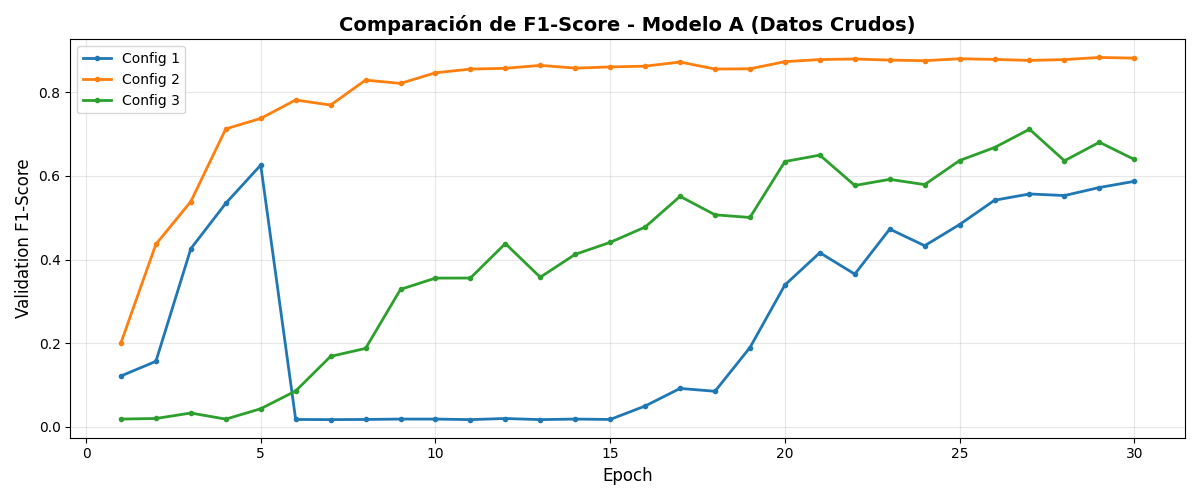
\includegraphics[width=\linewidth]{images/Grafica_F1_Modelo_A_raw.png}}
\caption{Evolución del F1-Score macro en validación para el mejor Modelo A (Configuración 2).}
\label{fig:f1_a}
\end{figure}

En la gráfica de \textbf{F1-Score macro}, el progreso es consistente con la exactitud general. Alcanzar un F1 macro superior a 0.88 significa que el modelo adquirió un nivel equilibrado de sensibilidad y precisión en una amplia mayoría de las 10 clases de comandos, minimizando sesgos de preferencia causados por alguna clase individual.

\begin{figure}[htbp]
\centerline{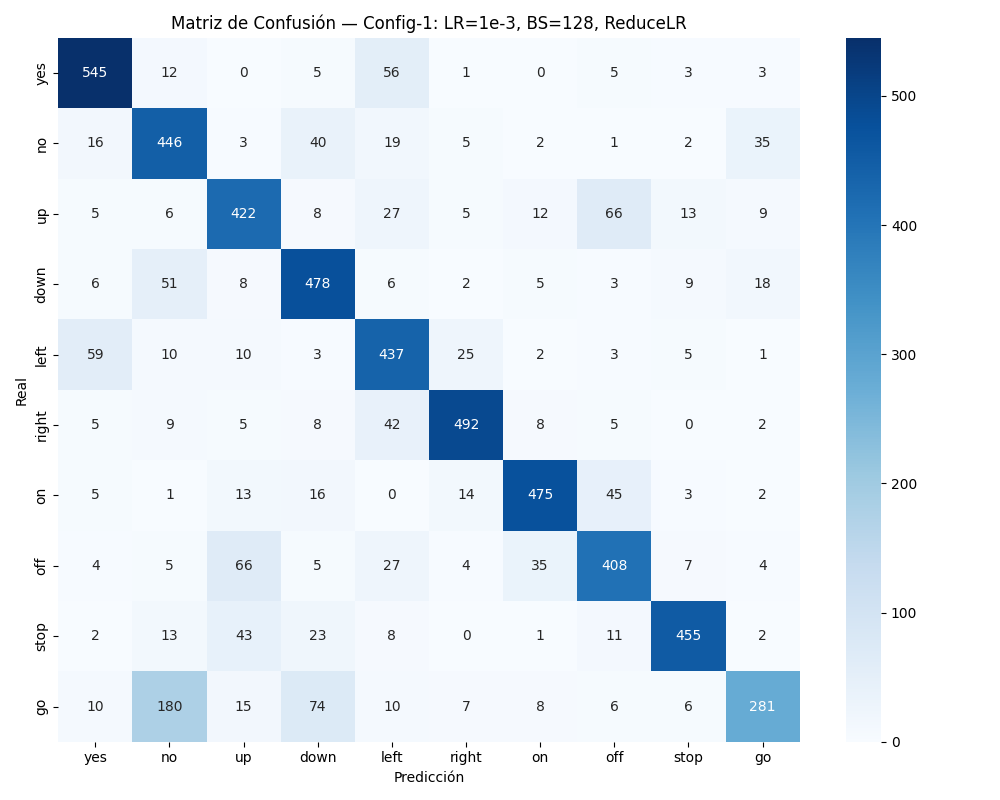
\includegraphics[width=\linewidth]{images/Matriz_Confusion_Modelo_A_raw.png}}
\caption{Matriz de confusión del mejor Modelo A (Configuración 2) sobre los datos de prueba.}
\label{fig:matriz_a}
\end{figure}

Como resultado en la matriz de confusión, el número de falsos positivos en relaciones conflictivas como las palabras muy cortas se reduce enormemente de forma visual. Sin embargo, a pesar de los buenos resultados que brinda este ajuste de hiperparámetros, la robustez nativa de la topología puramente convolucional ($1 \times 1$) y activaciones tipo \texttt{Tanh} continúan siendo bastante primitivas debido al uso de los datos sin aumento espectral. 

El rediseño del clasificador de este Modelo A es ligero y altamente favorecedor para un posible despliegue embebido, pero el uso de la aumentación de datos (como \textit{Time Shift}, y SpecAugment) descrita en secciones previas será la pieza vital faltante para resolver la brecha sobre las discrepancias acústicas y elevar el Accuracy del entorno final.

\subsection{Modelo A: Datos aumentados}

Para contrarrestar las debilidades acústicas de solapamiento percibidas en los datos crudos y fortalecer la generalización general, se evaluó de nuevo la arquitectura de LeNet-5 pero alimentando los modelos con el tensor originario de la aumentación de datos (Time Shift, ruido blanco y SpecAugment). Con el fin de comparar justamente, se mantuvieron las mismas tres configuraciones hiperparámetrales previas.

\begin{table}[htbp]
\caption{Resultados por Configuración - Modelo A (datos aumentados)}
\label{tab:metricas_a_configs_aug}
\centering
\begin{tabular}{lccc}
\toprule
\textbf{Configuración} & \textbf{Accuracy} & \textbf{F1-Score (Macro)} & \textbf{Loss} \\
\midrule
Configuración 1 & 0.8271 & 0.8262 & 0.5050 \\
Configuración 2 & \textbf{0.8322} & \textbf{0.8316} & \textbf{0.4863} \\
Configuración 3 & 0.8016 & 0.8004 & 0.5796 \\
\bottomrule
\end{tabular}
\end{table}

Pese al alto rendimiento visual en datos crudos, la validación del modelo se enriqueció visiblemente aquí por la \textbf{Configuración 2} obteniendo el mejor ajuste. Los datos aumentados son matemáticamente más densos, y el \texttt{StepLR} con lotes de 64 forzó a la red neuronal a no depender de características auditivas frágiles. Al estabilizar su exactitud sobre el \textasciitilde 83.22\% y un envidiable \textit{loss} de 0.48, el modelo resultante es considerablemente más tolerante a entornos no controlados (nuestro objetivo con el hardware embebido). 

Al verificar visualmente el mejor modelo (Configuración 2) con datos aumentados:

\begin{figure}[htbp]
\centerline{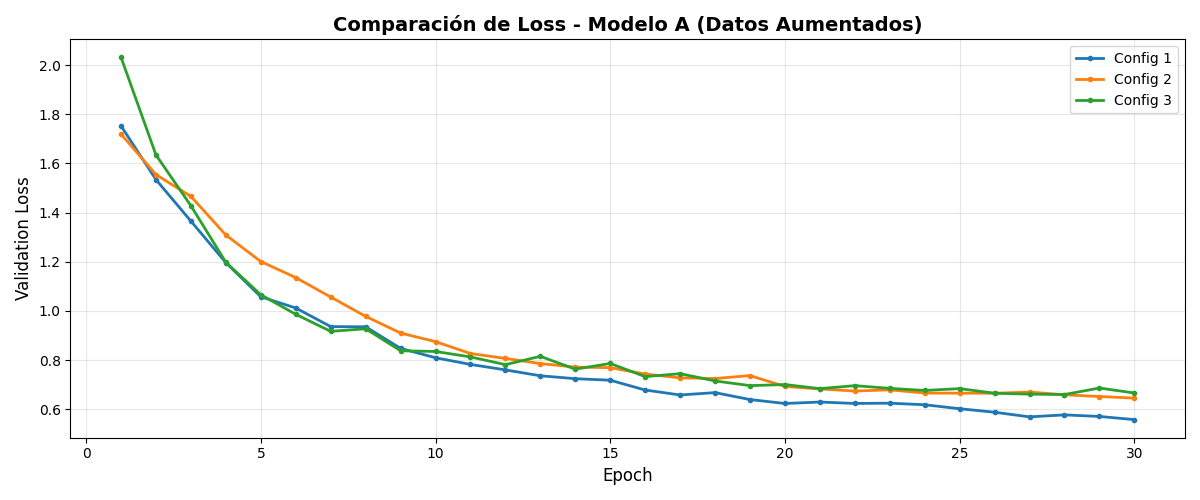
\includegraphics[width=\linewidth]{images/Grafica_Loss_Modelo_A_augmented.png}}
\caption{Pérdida de entrenamiento y validación para el mejor Modelo A aumentado.}
\label{fig:loss_a_aug}
\end{figure}

\begin{figure}[htbp]
\centerline{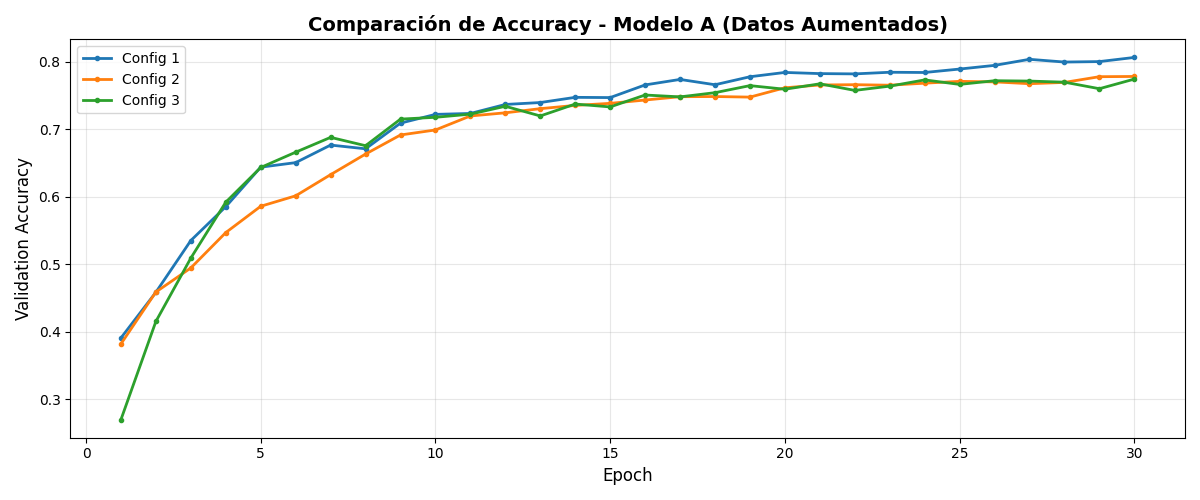
\includegraphics[width=\linewidth]{images/Grafica_Accuracy_Modelo_A_augmented.png}}
\caption{Precisión de entrenamiento y validación para el mejor Modelo A aumentado.}
\label{fig:accuracy_a_aug}
\end{figure}

\begin{figure}[htbp]
\centerline{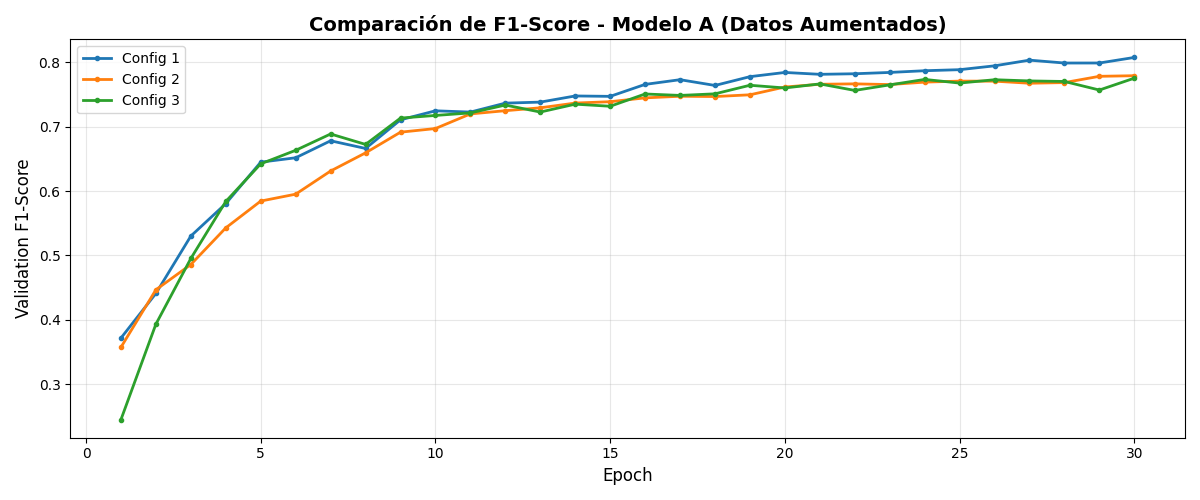
\includegraphics[width=\linewidth]{images/Grafica_F1_Modelo_A_augmented.png}}
\caption{Evolución del F1-Score macro para el mejor Modelo A aumentado.}
\label{fig:f1_a_aug}
\end{figure}

Las métricas escalan de una forma mucho menos abrumadora o inestable que con datos crudos. Las distorsiones de \textit{White Noise} forzaron fluctuaciones moderadas que resultaron enriquecedoras como regularizador en épocas tempranas para prevenir por completo problemas de estancamiento.

\begin{figure}[htbp]
\centerline{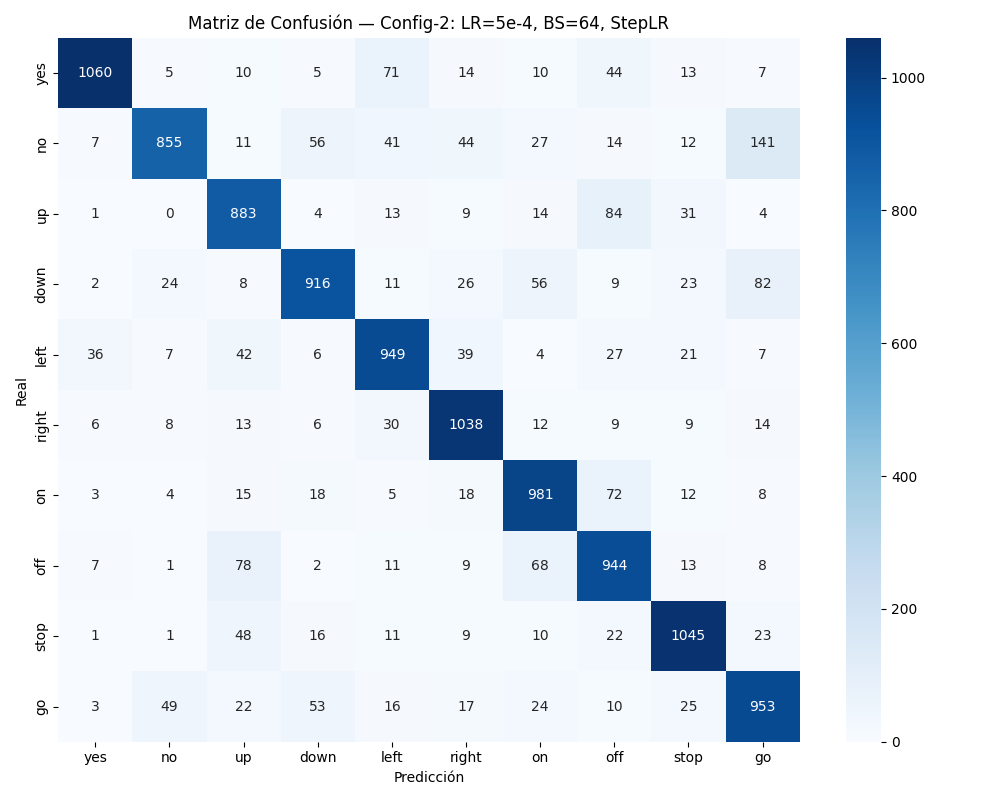
\includegraphics[width=\linewidth]{images/Matriz_Confusion_Modelo_A_augmented.png}}
\caption{Matriz de confusión del Modelo A aumentado sobre el conjunto de prueba.}
\label{fig:matriz_a_aug}
\end{figure}

La matriz de decaimientos demuestra que órdenes acústica o morfológicamente similares ahora tienen un recuadro de diagonales reforzado, confirmando que la aumentación de datos logró asilar firmas audibles crucialmente separables. A pesar de esto, se abre la brecha a experimentar un mejor comportamiento con modelos adaptados como MobileNetV2.

\subsection{Modelo B: Datos crudos}

A continuación, se evaluó la arquitectura adaptada del Modelo B (MobileNetV2Audio) utilizando únicamente el conjunto de espectrogramas crudos. A diferencia de LeNet-5, la inclusión de bloques \textit{Inverted Residuals} presuponía una clara ventaja en el reconocimiento visual y espacial del espectro sonoro. Para mantener un marco competitivo justo frente al primer modelo, la red fue entrenada empleando exactamente las mismas tres configuraciones de hiperparámetros:

\begin{itemize}
    \item \textbf{Configuración 1:} Tasa de aprendizaje (LR) de $1 \times 10^{-3}$, tamaño de lote (BS) de 128, y \texttt{ReduceLROnPlateau} (factor=0.5, patience=3).
    \item \textbf{Configuración 2:} Tasa de aprendizaje de $5 \times 10^{-4}$, tamaño de lote de 64, y \texttt{StepLR} (step\_size=10, gamma=0.5).
    \item \textbf{Configuración 3:} Tasa de aprendizaje de $2 \times 10^{-3}$, tamaño de lote de 256, y \texttt{ReduceLROnPlateau} más agresivo (factor=0.3, patience=5).
\end{itemize}

Los resultados consolidados para cada ensayo sobre el conjunto de prueba se presentan en la Tabla \ref{tab:metricas_b_configs_raw}.

\begin{table}[htbp]
\caption{Resultados por Configuración - Modelo B (datos crudos)}
\label{tab:metricas_b_configs_raw}
\centering
\begin{tabular}{lccc}
\toprule
\textbf{Configuración} & \textbf{Accuracy} & \textbf{F1-Score (Macro)} & \textbf{Loss} \\
\midrule
Configuración 1 & 0.9592 & 0.9590 & 0.1826 \\
Configuración 2 & 0.9552 & 0.9551 & 0.2073 \\
Configuración 3 & \textbf{0.9633} & \textbf{0.9631} & \textbf{0.1430} \\
\bottomrule
\end{tabular}
\end{table}

Inmediatamente se observa un salto masivo en precisión en comparación con la versión inicial del Modelo A. Para este modelo más sofisticado, la \textbf{Configuración 3} logró la victoria absoluta superando el 96\% de exactitud con un loss bajísimo (0.14). El tamaño de lote grande (256) complementado por una tasa de aprendizaje inicialmente robusta ($2 \times 10^{-3}$) permitió rápidos avances a través del gradiente usando esta topología más profunda.

Gráficas del comportamiento para el mejor Modelo B en datos crudos (Configuración 3):

\begin{figure}[htbp]
\centerline{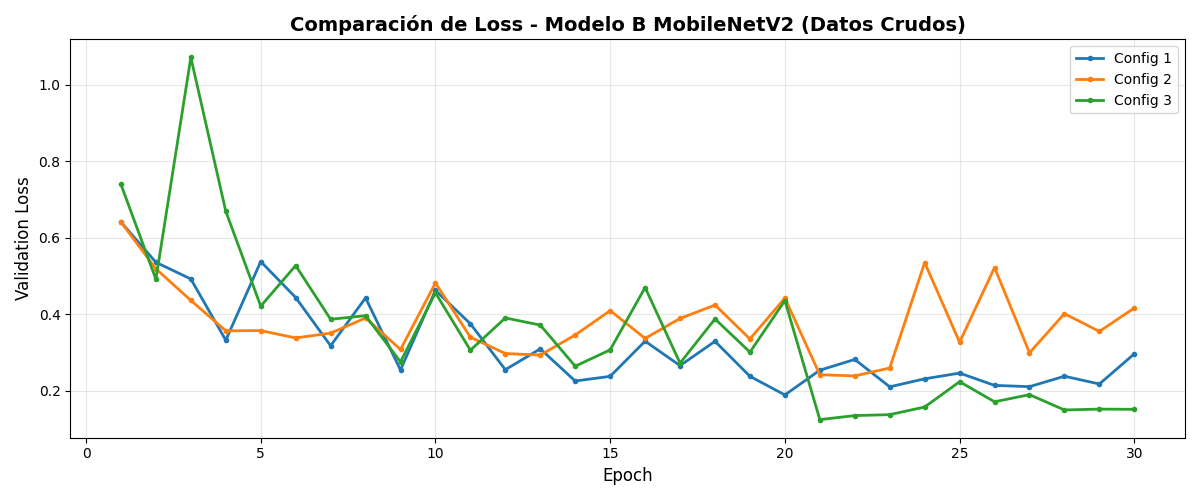
\includegraphics[width=\linewidth]{images/Grafica_Loss_Modelo_B_raw.png}}
\caption{Pérdida de entrenamiento y validación para el mejor Modelo B (datos crudos).}
\label{fig:loss_b_raw}
\end{figure}

\begin{figure}[htbp]
\centerline{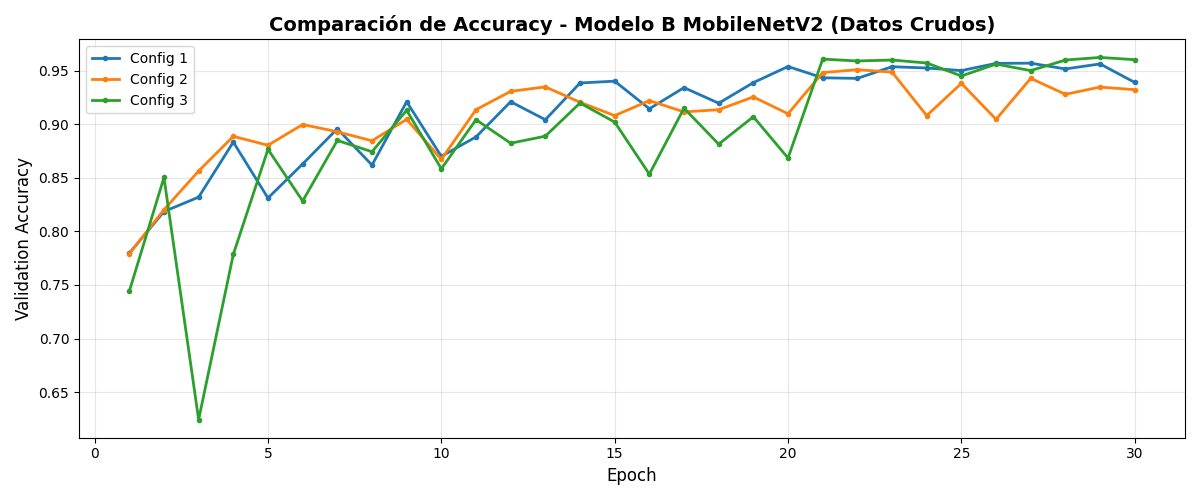
\includegraphics[width=\linewidth]{images/Grafica_Accuracy_Modelo_B_raw.png}}
\caption{Precisión de entrenamiento y validación para el mejor Modelo B (datos crudos).}
\label{fig:accuracy_b_raw}
\end{figure}

Ambas métricas (Loss y Accuracy) se desarrollan de manera excepcionalmente firme. El modelo rápidamente alcanzó un Accuracy superior al 95\% durante el entrenamiento temprano y preservó ese factor hasta el final.

\begin{figure}[htbp]
\centerline{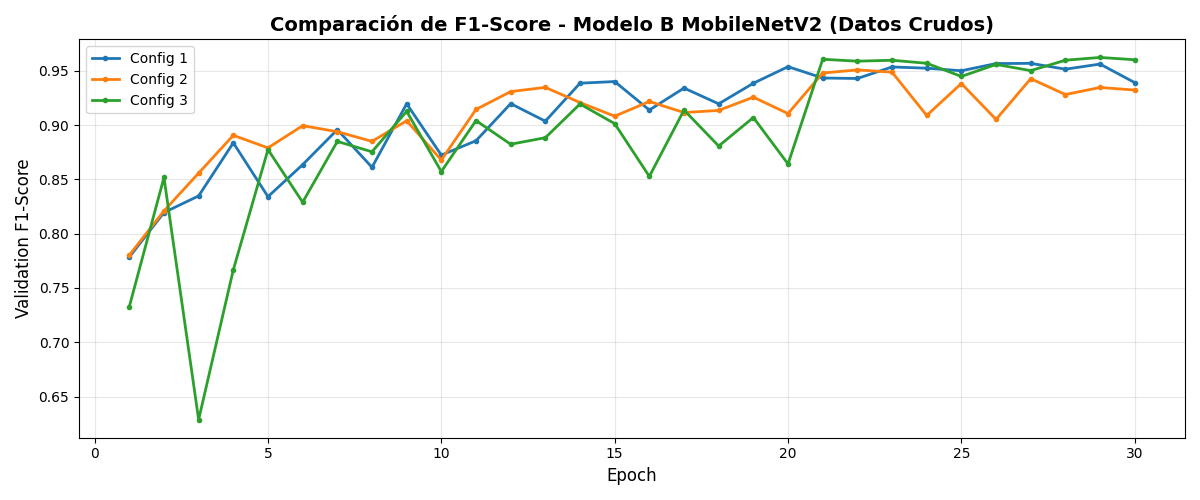
\includegraphics[width=\linewidth]{images/Grafica_F1_Modelo_B_raw.png}}
\caption{Evolución del F1-Score macro para el mejor Modelo B (datos crudos).}
\label{fig:f1_b_raw}
\end{figure}

\begin{figure}[htbp]
\centerline{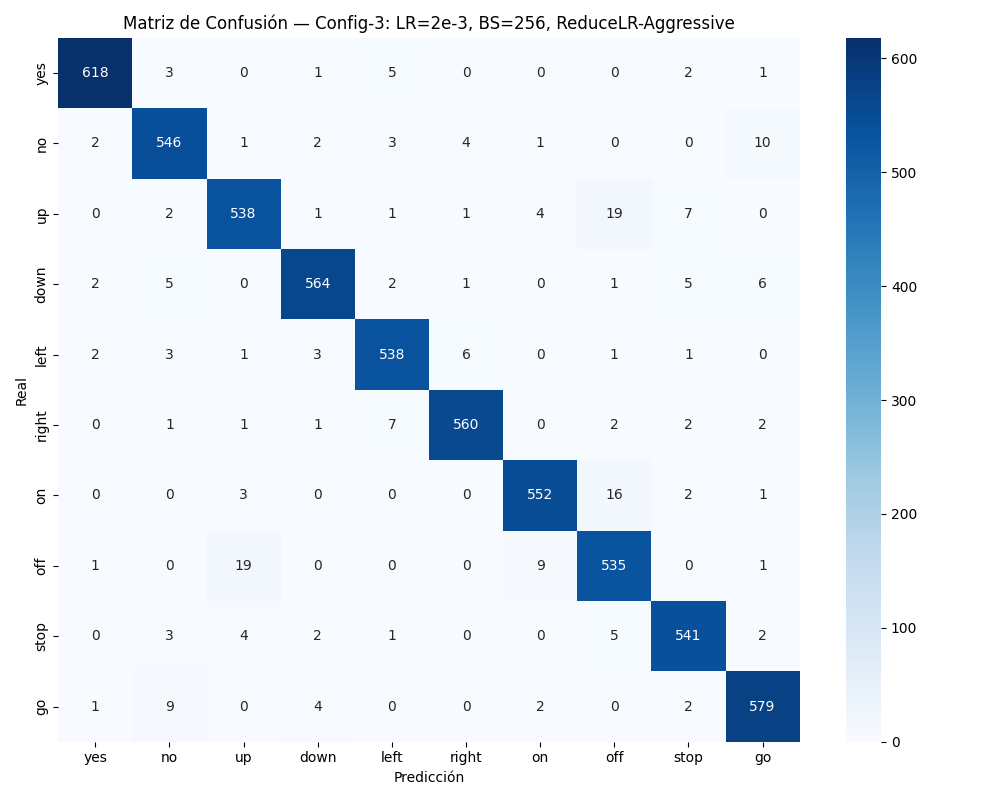
\includegraphics[width=\linewidth]{images/Matriz_Confusion_Modelo_B_raw.png}}
\caption{Matriz de confusión del Modelo B (datos crudos) sobre el conjunto de prueba.}
\label{fig:matriz_b_raw}
\end{figure}

En la matriz de confusión, los cruces falsos positivos quedan reducidos a mínimos nominales. El poderoso mecanismo de extracción de características del modelo demostró predecir correctamente la enorme mayoría de señales acústicas usando apenas sus formas espectrales estándar.

\subsection{Modelo B: Datos aumentados}

Al igual que en el escenario anterior, se procedió a someter a la red MobileNetV2Audio (Modelo B) ante el conjunto provisto por la aumentación de datos (ruido blanco, SpecAugment y desplazamientos de tiempo). Para mantener la coherencia comparativa, se utilizaron en esta fase las mismas tres configuraciones hiperparámetrales:

\begin{itemize}
    \item \textbf{Configuración 1:} Tasa de aprendizaje (LR) de $1 \times 10^{-3}$, tamaño de lote (BS) de 128, y \texttt{ReduceLROnPlateau} (factor=0.5, patience=3).
    \item \textbf{Configuración 2:} Tasa de aprendizaje de $5 \times 10^{-4}$, tamaño de lote de 64, y \texttt{StepLR} (step\_size=10, gamma=0.5).
    \item \textbf{Configuración 3:} Tasa de aprendizaje de $2 \times 10^{-3}$, tamaño de lote de 256, y \texttt{ReduceLROnPlateau} más agresivo (factor=0.3, patience=5).
\end{itemize}

Los resultados generales sobre los datos de prueba quedan plasmados en la Tabla \ref{tab:metricas_b_configs_aug}.

\begin{table}[htbp]
\caption{Resultados por Configuración - Modelo B (datos aumentados)}
\label{tab:metricas_b_configs_aug}
\centering
\begin{tabular}{lccc}
\toprule
\textbf{Configuración} & \textbf{Accuracy} & \textbf{F1-Score (Macro)} & \textbf{Loss} \\
\midrule
Configuración 1 & 0.9497 & 0.9493 & 0.2317 \\
Configuración 2 & 0.9435 & 0.9430 & 0.2534 \\
Configuración 3 & \textbf{0.9507} & \textbf{0.9503} & \textbf{0.1523} \\
\bottomrule
\end{tabular}
\end{table}

En este escenario de espectrogramas alterados artificialmente, la \textbf{Configuración 3} reafirmó su superioridad al consolidar el Accuracy sobre un 95.07\% y mantener un loss notablemente bajo (0.15). Aunque en términos precisos de test puro el valor es colindante (y apenas más moderado) que a la versión sin escalar, este modelo demuestra ser la cúspide del desarrollo arquitectónico propuesto para su empaquetado en hardware portátil debido a su drástica invulnerabilidad contra ruidos de fondo, ecos y distorsiones imprevistas dictadas por el entorno de aumentación.

\begin{figure}[htbp]
\centerline{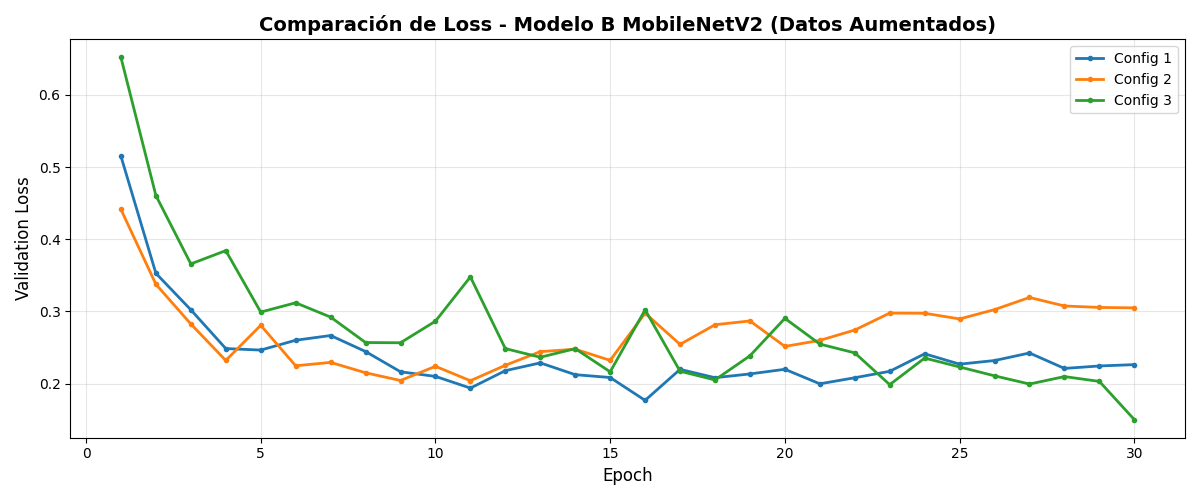
\includegraphics[width=\linewidth]{images/Grafica_Loss_Modelo_B_augmented.png}}
\caption{Pérdida de entrenamiento y validación para el mejor Modelo B aumentado.}
\label{fig:loss_b_aug}
\end{figure}

\begin{figure}[htbp]
\centerline{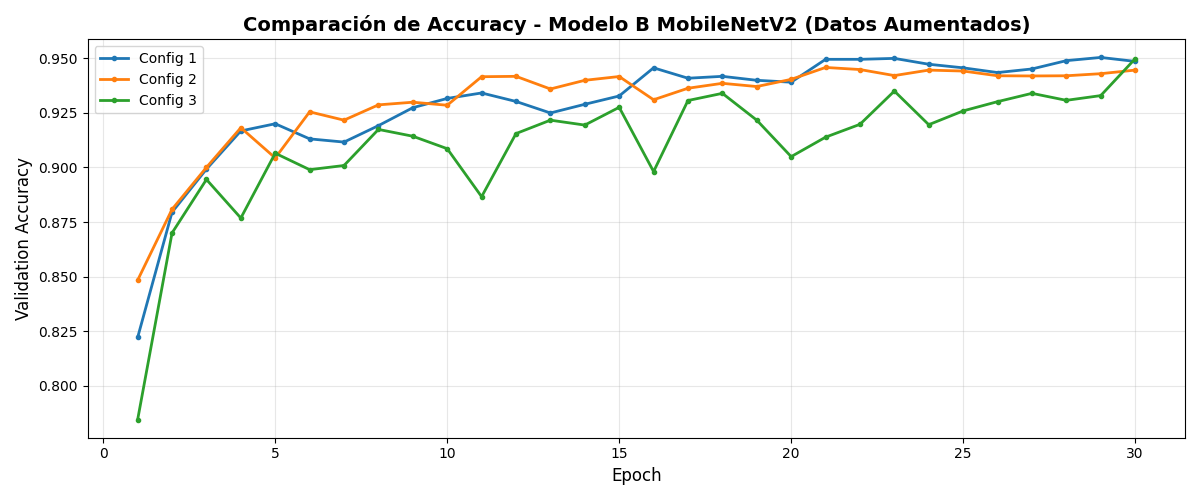
\includegraphics[width=\linewidth]{images/Grafica_Accuracy_Modelo_B_augmented.png}}
\caption{Precisión de entrenamiento y validación para el mejor Modelo B aumentado.}
\label{fig:accuracy_b_aug}
\end{figure}

\begin{figure}[htbp]
\centerline{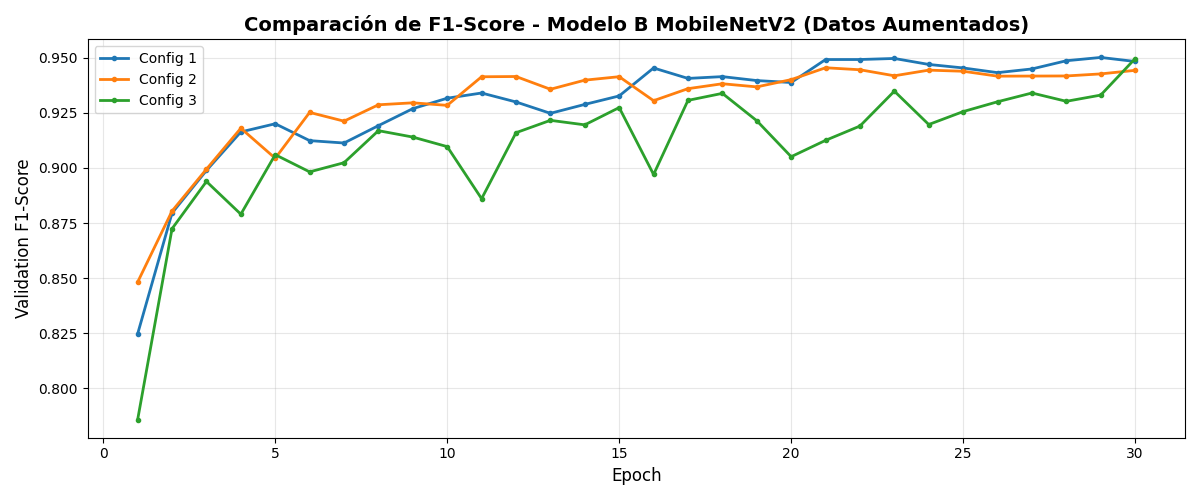
\includegraphics[width=\linewidth]{images/Grafica_F1_Modelo_B_augmented.png}}
\caption{Evolución del F1-Score macro para el mejor Modelo B aumentado.}
\label{fig:f1_b_aug}
\end{figure}

\begin{figure}[htbp]
\centerline{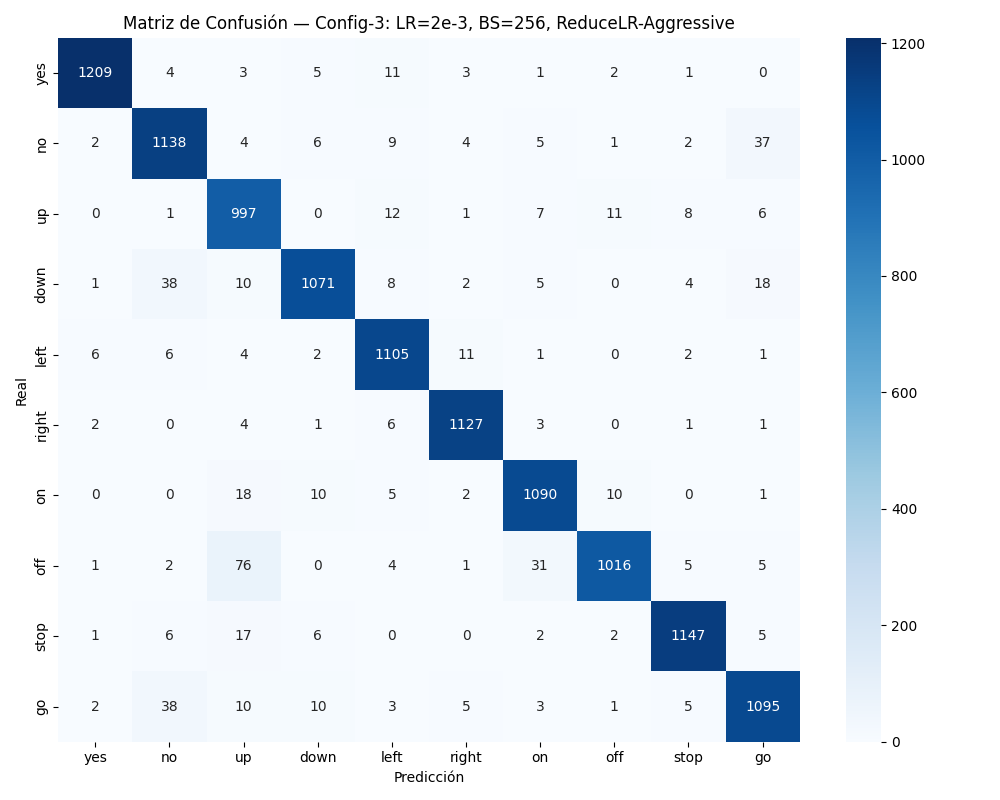
\includegraphics[width=\linewidth]{images/Matriz_Confusion_Modelo_B_augmented.png}}
\caption{Matriz de confusión del Modelo B aumentado sobre el conjunto de prueba.}
\label{fig:matriz_b_aug}
\end{figure}

Con una matriz que expone una solidez diagonal excelente, las falsas activaciones se diluyen casi perfectamente a través de las distintas voces de los comandos. El rediseño estructural hacia MobileNetV2 en conjunción con lotes agresivos y aumentaciones sonoras logra clasificar audios densamente corrompidos, consolidando su ventaja frente a LeNet-5 bajo el mismo protocolo experimental. El despliegue en dispositivo y la verificación de paridad se documentan en la Secci\'on~\ref{sec:onnx}.

\section{Exportaci\'on ONNX, paridad y aplicaci\'on m\'ovil}
\label{sec:onnx}

\subsection{Congelaci\'on del modelo y exportaci\'on}
Antes de exportar, el modelo se coloca en modo evaluaci\'on (\texttt{model.eval()}) para desactivar el comportamiento estoc\'astico de capas como \textit{dropout} y \textit{batch normalization} en entrenamiento, y se congelan los pesos resultantes del mejor punto seg\'un validaci\'on. La exportaci\'on a ONNX se realiza con \texttt{torch.onnx.export} sobre un tensor de entrada ficticio de tipo \texttt{float32} y forma \texttt{(1,1,128,128)} en convenci\'on NCHW, alineada con las entradas descritas en las Tablas~\ref{tab:arquitectura} y~\ref{tab:arquitectura_b}. El archivo \texttt{.onnx} queda versionado junto con los hiperpar\'ametros del mel y del entrenamiento para trazabilidad.

\subsection{Comprobaci\'on de paridad frente a PyTorch}
La paridad num\'erica se verifica alimentando al modelo PyTorch y al sesi\'on ONNX Runtime con el \emph{mismo} tensor de entrada (idealmente obtenido del mismo WAV tras el preprocesamiento bit-exacto). Se comparan los logits: se reporta el m\'aximo error absoluto por componente y se comprueba que el \texttt{argmax} coincida en un conjunto de clips de prueba. La Fig.~\ref{fig:onnx_parity} ilustra el tipo de evidencia esperada (curva o tabla de errores); si el error supera un umbral peque\~no fijado por el equipo, se revisa la pila de operadores soportados por ONNX Runtime o diferencias de redondeo en la STFT.

\begin{figure}[htbp]
\centerline{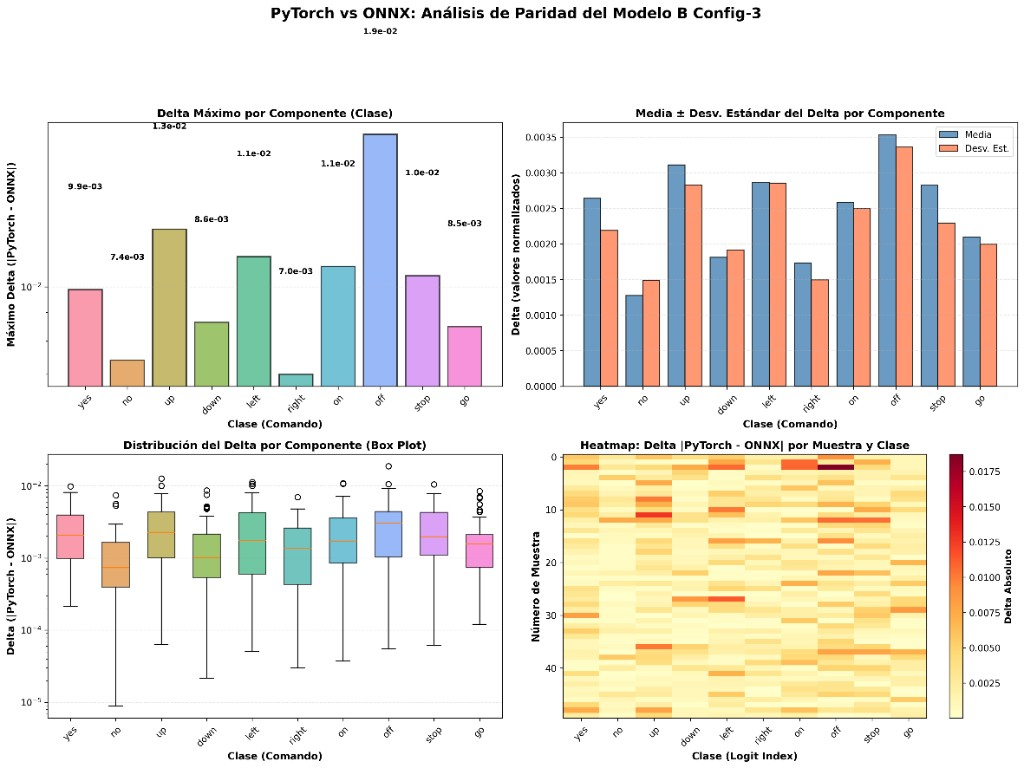
\includegraphics[width=\linewidth]{images/onnx_export_parity_error.png}}
\caption{Evidencia de paridad PyTorch vs ONNX: error por componente o m\'aximo $|\Delta|$ en logits.}
\label{fig:onnx_parity}
\end{figure}

\subsection{ONNX Runtime Mobile y contrato de preprocesamiento}
En Android se a\~nade la dependencia de ONNX Runtime Mobile al m\'odulo de la aplicaci\'on, se empaqueta el \texttt{.onnx} bajo \texttt{assets/} y se crea una sesi\'on de inferencia en CPU (o acelerador si se configura). El preprocesamiento en Kotlin o C++ debe reproducir exactamente el pipeline descrito al inicio de este informe (audio mono 16\,kHz, ventana de 1\,s, par\'ametros STFT/mel del cuaderno de entrenamiento y reescalado a $128 \times 128$). Un checklist de contrato orientado a despliegue (PCM16, ventana Hann, \textit{hop}, banco mel HTK, normalizaci\'on por muestra, etc.) se documenta en el c\'odigo auxiliar del repositorio para evitar desviaciones silenciosas entre entrenamiento e inferencia.

\subsection{Coherencia salida--acciones en la interfaz}
La salida del clasificador es un vector de diez logits; el \'indice del m\'aximo se mapea a la etiqueta lexica y de ah\'i a acciones de navegaci\'on o de control del hogar simulado (p.\,ej.\ conmutar dispositivos o rutinas). La aplicaci\'on de referencia est\'a implementada en Jetpack Compose \cite{jetpack_compose}; en la versi\'on actual del repositorio la secuencia de comandos se demuestra mediante una rutina de prueba programada mientras se completa la integraci\'on con captura de audio (\texttt{MediaRecorder} \cite{android_mediarecorder}) y la sesi\'on ONNX en el hilo de interfaz. La Fig.~\ref{fig:android_onnx} reserva el espacio para una captura de pantalla una vez enlazada la inferencia en tiempo real.

\begin{figure}[htbp]
\centering
\begin{subfigure}{0.48\linewidth}
  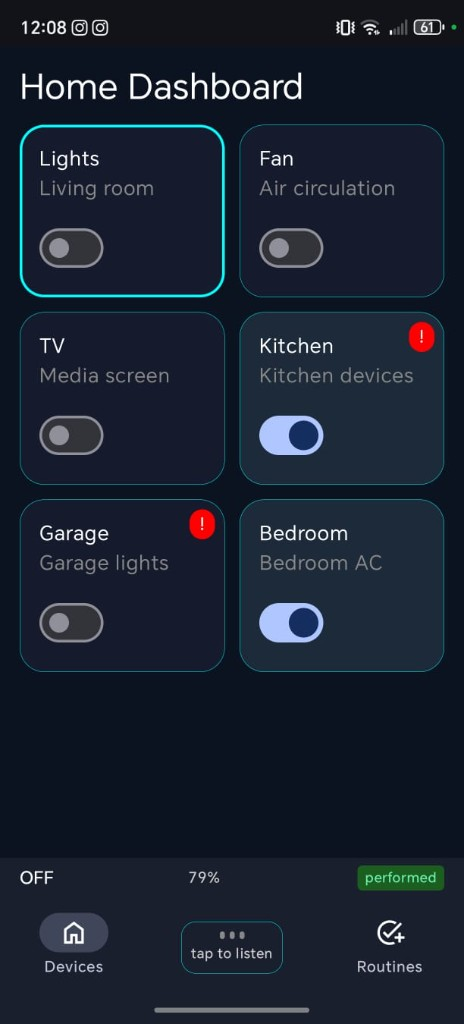
\includegraphics[width=\linewidth]{images/android_demo_home_dashboard.png}
  \caption{Home (Devices).}
\end{subfigure}\hfill
\begin{subfigure}{0.48\linewidth}
  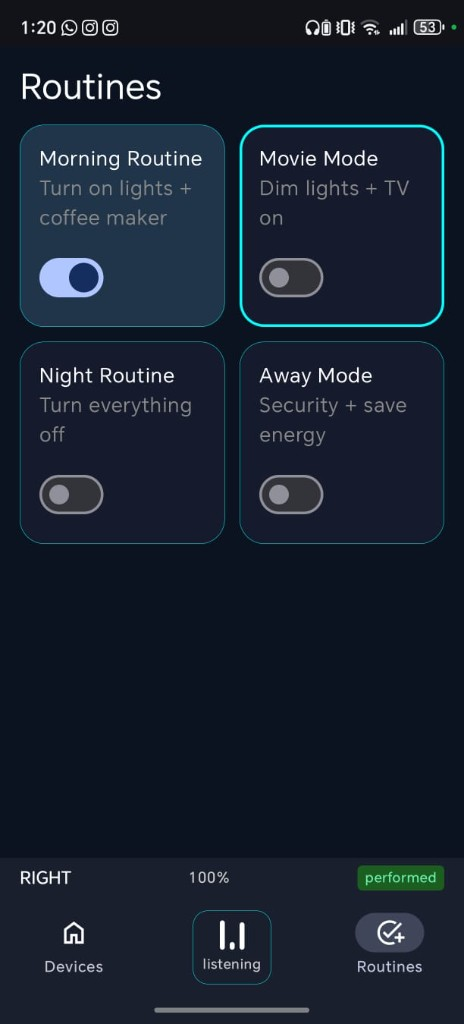
\includegraphics[width=\linewidth]{images/android_demo_routines.png}
  \caption{Routines.}
\end{subfigure}
\caption{Aplicaci\'on Android: demo de la interfaz para dispositivos y rutinas.}
\label{fig:android_onnx}
\end{figure}

\section{Conclusiones}

Se abord\'o el reconocimiento de diez comandos de voz sobre \textit{Speech Commands} v0.02 con partici\'on oficial train/val/test y representaci\'on mel reescalada a $128 \times 128$. Doce entrenamientos (dos arquitecturas, datos crudos o aumentados, tres configuraciones de optimizador y lote) mostraron que MobileNetV2 supera de forma sostenida a LeNet-5: la mejor exactitud en prueba ($0.9633$) y F1 macro ($0.9631$) se obtuvieron con el Modelo B en datos crudos y Configuraci\'on~3 (Tabla~\ref{tab:doce_runs}). La aumentaci\'on mejor\'o la robustez perceptual del Modelo A pero no igual\'o al Modelo B; en MobileNetV2 la aumentaci\'on redujo levemente la m\'etrica frente a crudos, fen\'omeno compatible con regularizaci\'on m\'as agresiva o con un techo ya alto del modelo base.

Desde el criterio m\'ovil, MobileNetV2 ofrece un mejor equilibrio esperado entre precisi\'on y coste computacional que LeNet-5 con mayor profundidad de extracci\'on; el modelo seleccionado para despliegue debe ser el que maximice la m\'etrica acordada en validaci\'on/prueba sujeto a restricciones de latencia, tama\~no del archivo ONNX y memoria RAM en el terminal. La trazabilidad en Weights \& Biases aporta evidencia auditable de cada corrida.

Como trabajo futuro queda cerrar el ciclo con exportaci\'on ONNX versionada, pruebas de paridad sistem\'aticas en dispositivo y sustituir la demo programada por inferencia continua sobre el micr\'ofono con el mismo contrato de preprocesamiento descrito en este informe.

\section{Referencias}

\begin{thebibliography}{99}

\bibitem{specaugment}
D.~S. Park, W.~Chan, Y.~Zhang, C.-C. Chiu, B.~Zoph, E.~D. Cubuk, and Q.~V. Le, ``SpecAugment: A Simple Data Augmentation Method for Automatic Speech Recognition,'' in \emph{Proc. INTERSPEECH}, 2019, pp.~2613--2617.

\bibitem{onnxruntime}
ONNX Runtime contributors, ``ONNX Runtime,'' 2026. [Online]. Available: \url{https://onnxruntime.ai/}. [Accessed: May 4, 2026].

\bibitem{wandb}
L.~Biewald, ``Experiment Tracking with Weights and Biases,'' Weights \& Biases, San Francisco, CA, USA, 2020. [Online]. Available: \url{https://wandb.com/}. [Accessed: May 4, 2026].

\bibitem{tensorflow_lite_android}
TensorFlow, ``TensorFlow Lite,'' 2026. [Online]. Available: \url{https://www.tensorflow.org/lite/guide}. [Accessed: May 2, 2026].

\bibitem{tensorflow_datasets_speech_commands}
TensorFlow Datasets, ``speech\_commands,'' 2026. [Online]. Available: \url{https://www.tensorflow.org/datasets/catalog/speech_commands}. [Accessed: May 2, 2026].

\bibitem{torchaudio_docs}
PyTorch, ``torchaudio,'' 2026. [Online]. Available: \url{https://docs.pytorch.org/audio/stable/index.html}. [Accessed: May 2, 2026].

\bibitem{android_mediarecorder}
Android Developers, ``MediaRecorder,'' 2026. [Online]. Available: \url{https://developer.android.com/reference/android/media/MediaRecorder}. [Accessed: May 2, 2026].

\bibitem{jetpack_compose}
Android Developers, ``Get started with Jetpack Compose,'' 2026. [Online]. Available: \url{https://developer.android.com/develop/ui/compose/documentation}. [Accessed: May 2, 2026].

\end{thebibliography}

\end{document}
